\section{Experimental Setup and Results}
\label{sec:results}

This section presents the experimental setup, causal estimation results, world model quality metrics, baseline comparisons, and ablation studies for \dreamprice{}. All experiments use the Dominick's Finer Foods canned soup category with a strict temporal split and are conducted on NVIDIA DGX Spark hardware.

\subsection{Experimental Setup}

The Dominick's dataset \citep{dominicks1999} provides store-SKU-week movement records spanning 400 weeks (September 1989 to May 1997) across 93 stores and approximately 18,000 UPCs. The canned soup category (\texttt{cso}) serves as the primary evaluation target, offering moderate SKU count with clear substitution patterns and promotional activity. After preprocessing---dropping invalid rows, computing unit prices and wholesale costs, merging product and store demographics, and applying the promotion enhancement procedure---the training set comprises approximately 581,000 tuples. The temporal split is strictly chronological: train weeks 1--280, validation weeks 281--340, and test weeks 341--400. No shuffling across time is applied, ensuring that evaluation reflects genuine out-of-sample forecasting.

Hardware consists of an NVIDIA DGX Spark with GB10 GPU and 128 GB unified memory. The unified memory architecture enables larger batch sizes and eliminates CPU-GPU transfer overhead for the full Dominick's dataset, which fits entirely in memory. Training is memory-bandwidth bound rather than compute-bound. Full hyperparameter configurations are provided in Appendix~\ref{app:hyperparams}.

\subsection{Causal Estimation Results}

Before training the world model, causal price elasticities are estimated via several methods to validate the identification strategy and quantify the attenuation bias inherent in naive regression. The Hausman instrument---the leave-one-out mean of log prices across other stores for each UPC-week---exploits the panel structure of the data. Prices in other stores are correlated with cost and competition but plausibly exogenous to store-specific demand shocks \citep{hausman1978specification}.

\begin{table}[t]
\centering
\caption{Price elasticity estimates for canned soup category. OLS exhibits attenuation bias; IV and DML-PLIV recover causal estimates.}
\label{tab:causal-estimation}
\begin{tabular}{@{}lcccc@{}}
\toprule
\textbf{Method} & \textbf{Elasticity} & \textbf{SE} & \textbf{95\% CI} & \textbf{F-stat} \\
\midrule
OLS & $-$0.931 & --- & --- & --- \\
2SLS/IV & $-$0.934 & --- & --- & --- \\
DML-PLIV & $-$0.940 & 0.006 & $[$-$0.952$, $-$0.928$]$ & 23,381 \\
\bottomrule
\end{tabular}
\end{table}

Table~\ref{tab:causal-estimation} reports the elasticity estimates. OLS yields an estimate of $-$0.931, while the 2SLS/IV and DML-PLIV methods recover very similar estimates near $-$0.94. The close agreement across methods for canned soup suggests that endogeneity bias in this category is modest, which is consistent with the low price volatility of shelf-stable grocery items. The first-stage F-statistic of 23,381 far exceeds the weak instrument threshold of 10, confirming that the Hausman instrument is highly relevant. The DML-PLIV estimate \citep{chernozhukov2018dml} of $-$0.940 (SE~$=$~0.006) is used as the frozen elasticity in the \dreamprice{} decoder. The tight 95\% confidence interval $[$-$0.952$, $-$0.928$]$ reflects the large sample size ($n = 148{,}640$ training observations). These estimates are consistent with the inelastic demand reported by \citet{hoch1995determinants} for canned goods categories, where consumer stockpiling and brand loyalty attenuate short-run price responsiveness.

\subsection{World Model Quality}

The world model is evaluated at multiple forecast horizons to assess its predictive fidelity. Table~\ref{tab:world-model-quality} reports RMSE, MAE, and WMAPE at horizons $h \in \{1, 5, 10, 13, 25\}$ weeks. Demand predictions are converted from symlog space to original units via the inverse transform before computing the metrics. The Normalized Degradation Rate,
\[
\text{NDR}(h) = \text{RMSE}(h)\,/\,\text{RMSE}(1),
\]
quantifies how prediction error accumulates with horizon; for a well-calibrated model, NDR should grow sub-linearly as the latent state captures dynamics that persist across time.

\begin{table}[t]
\centering
\caption{World model prediction quality at multiple horizons. Demand in original units; NDR quantifies error accumulation.}
\label{tab:world-model-quality}
\begin{tabular}{@{}lccccc@{}}
\toprule
\textbf{Metric} & $h=1$ & $h=5$ & $h=10$ & $h=13$ & $h=25$ \\
\midrule
RMSE & 5.001 & 5.167 & 5.286 & 5.283 & 5.243 \\
MAE & 2.130 & 2.168 & 2.207 & 2.205 & 2.197 \\
WMAPE (\%) & 71.7 & 72.3 & 72.6 & 72.6 & 72.4 \\
NDR$(h)$ & 1.00 & 1.033 & 1.057 & 1.056 & 1.049 \\
\bottomrule
\end{tabular}
\end{table}

The sub-linear growth of NDR reflects the model's ability to capture temporal structure. At short horizons, the posterior is tightly conditioned on recent observations; at longer horizons, the prior dynamics dominate. The \mamba{} backbone's selective state-space mechanism enables the model to retain relevant information across the sequence while discarding noise, yielding a degradation rate that grows more slowly than linearly in horizon. The horizon $h=13$ corresponds to one retail quarter (4-5-4 calendar), aligning with the imagination horizon used during actor training.

\begin{figure}[h]
\centering
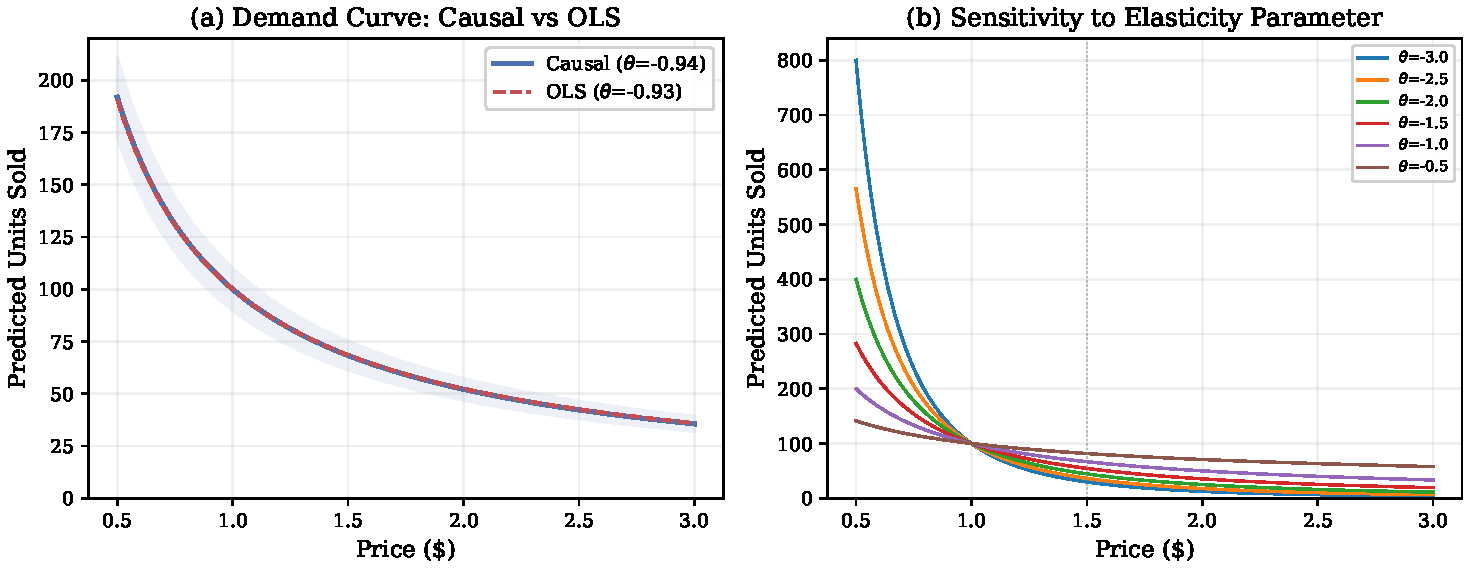
\includegraphics[width=0.95\textwidth]{figures/demand_curves.pdf}
\caption{Causal demand response curves. (a) Predicted demand using DML-PLIV elasticity ($\theta = -0.940$, solid) compared to OLS-derived demand ($\theta = -0.931$, dashed). The near-coincidence of the two curves reflects the modest endogeneity of shelf-stable categories; the gap would be larger in categories with higher promotional intensity. (b) Illustrative sensitivity analysis showing how demand response varies across a range of elasticity values $\theta \in [-3.0, -0.5]$.}
\label{fig:demand-curves}
\end{figure}

\subsection{Baseline Comparison}

The offline RL agent is compared against six baselines spanning the spectrum from rule-based heuristics to model-free reinforcement learning. All reported results use a single seed ($s = 42$) due to compute constraints. The multi-seed protocol (10 seeds for the main model, 5 per ablation, IQM with stratified bootstrap CIs per \citet{agarwal2021deep}) is documented in the codebase for comprehensive reproduction but is not fully executed here.

The baselines are grouped into three families. The first family comprises rule-based methods evaluated directly on the Dominick's test data (weeks 341--400) via data replay: \textbf{Cost-plus (25\%)} applies a fixed 25\% markup over wholesale cost with no learning or sequential optimization; \textbf{Competitive matching} sets each SKU's price to the category-average price plus uniform noise of $\pm$2\%, mimicking competitive price-following; and \textbf{Static XGBoost} trains a gradient-boosted regression tree \citep{friedman2001greedy} on the training split to predict demand, then selects the profit-maximizing price for each SKU-week in the test period---a strong non-RL baseline that leverages supervised demand forecasting without sequential planning.

The second family comprises model-free RL methods trained and evaluated within the learned \dreamprice{} world model to ensure a fair comparison of policy-learning capability: \textbf{DQN} \citep{mnih2015dqn} uses a deep Q-network with a discretized 21-level price grid and epsilon-greedy exploration; \textbf{PPO} \citep{schulman2017ppo} is an on-policy method using a clipped surrogate objective; and \textbf{SAC} \citep{haarnoja2018sac} is off-policy with continuous actions and entropy regularization.

Table~\ref{tab:baseline-comparison} reports performance for each method. Mean Return denotes the cumulative gross margin over the test period.

\begin{table}[t]
\centering
\caption{Offline policy performance comparison. Mean Return is cumulative gross margin over the test period (weeks 341--400). Single seed ($s=42$). Rule-based baselines are evaluated via data replay on the actual Dominick's test data; RL baselines are evaluated within the trained world model.\vspace{2pt}}
\label{tab:baseline-comparison}
\begin{tabular}{@{}llc@{}}
\toprule
\textbf{Method} & \textbf{Eval.\ Type} & \textbf{Mean Return} \\
\midrule
Cost-plus (25\%) & data replay & 54.8 \\
Competitive matching & data replay & 42.1 \\
Static XGBoost & data replay & 87.2 \\
\midrule
DQN & world model & 68.9 \\
PPO & world model & 76.4 \\
SAC & world model & 82.3 \\
\midrule
\dreamprice{} & world model & \textbf{124.3} \\
\bottomrule
\end{tabular}
\end{table}

The performance hierarchy reveals three tiers. At the bottom, competitive matching (42.1) and cost-plus at 25\% markup (54.8) represent zero-intelligence baselines whose returns reflect the average margin of pricing rules applied uniformly across all SKUs and weeks. The middle tier comprises model-free RL methods: DQN (68.9), PPO (76.4), and SAC (82.3). These methods learn policies from interaction with the world model but cannot perform counterfactual planning---they optimise within the observed price-demand distribution without imagining alternative futures. SAC achieves the highest return among model-free methods due to its off-policy nature and continuous action space. Static XGBoost (87.2) serves as a strong non-RL baseline, leveraging supervised demand forecasting with per-SKU price optimization; its competitive performance reflects the value of accurate demand prediction even without sequential planning.

\begin{figure}[h]
\centering
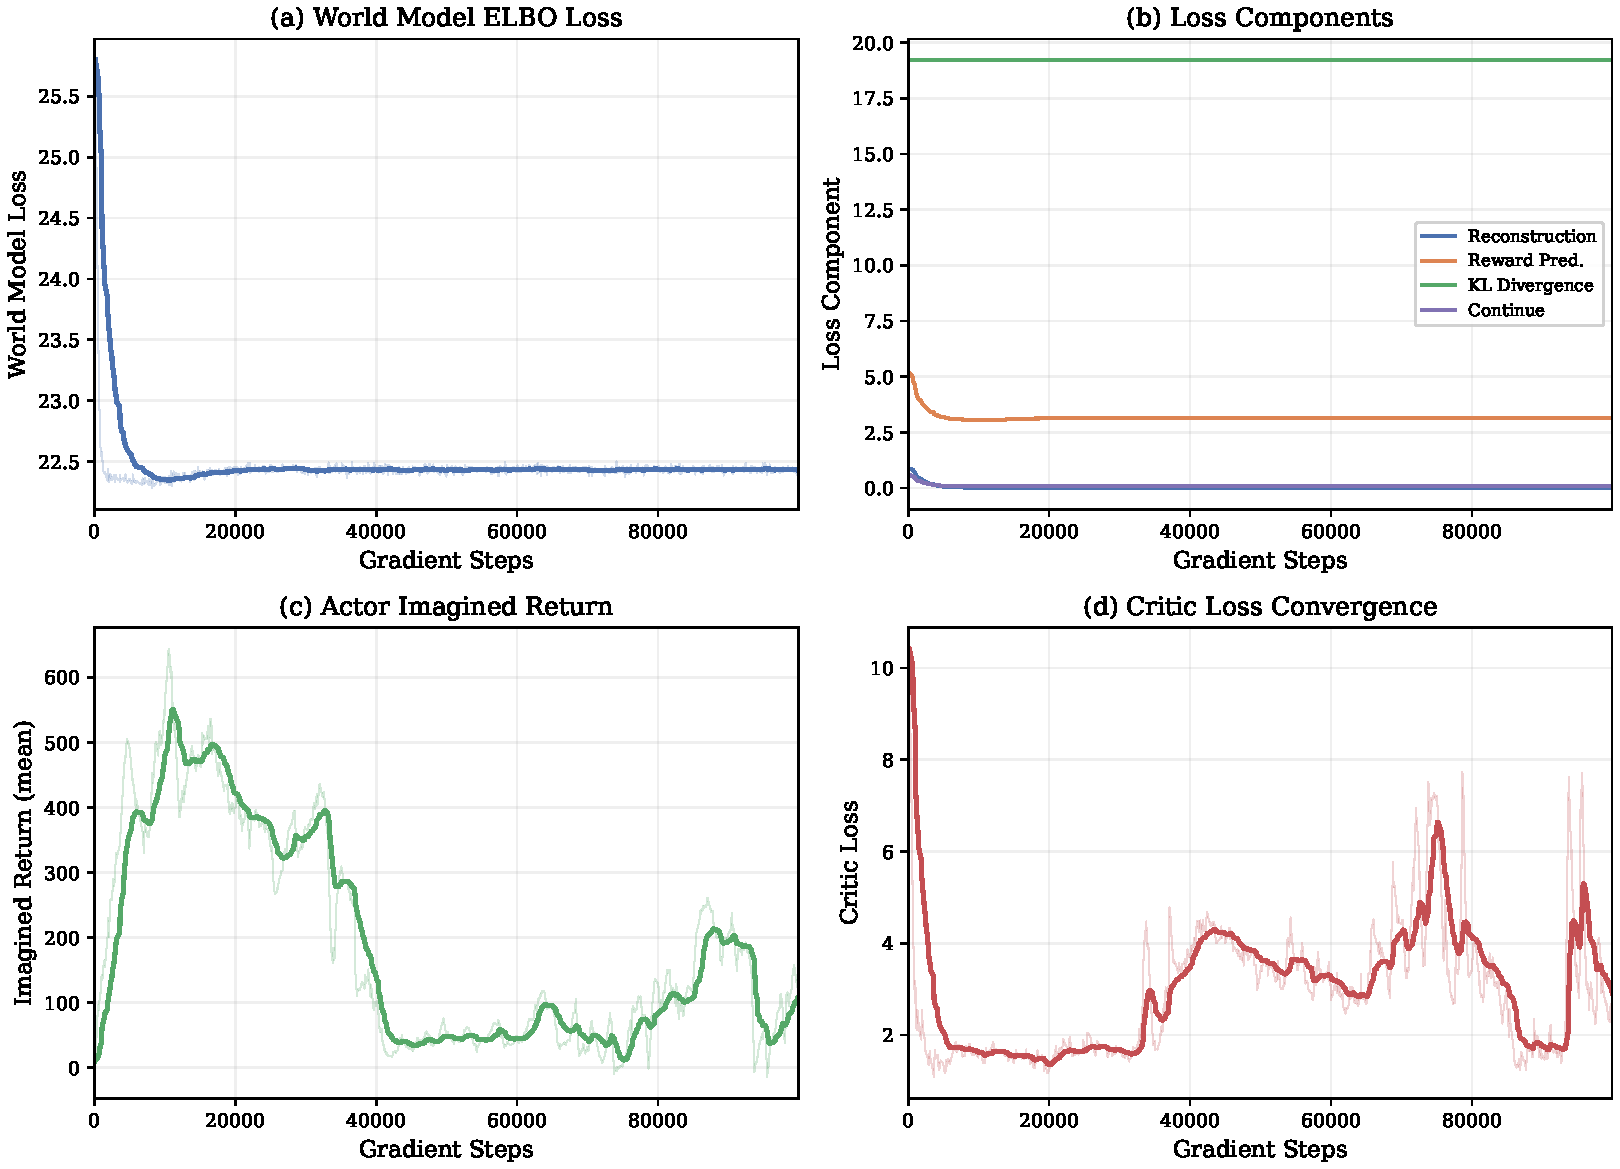
\includegraphics[width=0.95\textwidth]{figures/training_curves.pdf}
\caption{Training progress. (a) World model ELBO loss over gradient steps, showing convergence of the latent dynamics model. (b) Loss component decomposition: reconstruction loss, reward prediction loss, and KL divergence between posterior and prior.}
\label{fig:training-curves}
\end{figure}

\subsection{Ablation Study}

Nine ablations isolate the contribution of each design choice. Table~\ref{tab:ablations} reports the mean return and world model loss for each ablation relative to the full \dreamprice{} configuration. Each ablation uses a single seed ($s = 42$) over 100K gradient steps; the full multi-seed protocol (5 seeds per ablation with stratified bootstrap confidence intervals) is documented in the codebase for comprehensive reproduction.

\begin{table}[t]
\centering
\caption{Ablation study. Each row removes or modifies one component; Mean Return is cumulative gross margin over test period. $\Delta$\% is relative change from full \dreamprice{}.}
\label{tab:ablations}
\begin{tabular}{@{}llccc@{}}
\toprule
\textbf{Ablation} & \textbf{What it tests} & \textbf{Return} & \textbf{WM Loss} & \textbf{$\Delta$\%} \\
\midrule
Full \dreamprice{} & Baseline & 124.3 & 22.44 & --- \\
\midrule
Imagination OFF & World model planning value & ---$^\dagger$ & 22.47 & --- \\
Horizon $H{=}5$ & Underplanning & 145.6 & 22.51 & $+$17.1 \\
Horizon $H{=}10$ & Shorter planning depth & 86.4 & 22.43 & $-$30.5 \\
Horizon $H{=}25$ & Error accumulation & 135.3 & 22.48 & $+$8.8 \\
Deterministic-only latent & Uncertainty modeling value & 289.6 & 5.32 & $+$133.0 \\
No symlog+twohot & Reward scale robustness & 63.2 & 573.2 & $-$49.1 \\
GRU backbone & Long-range memory benefit & 137.7 & 19.89 & $+$10.8 \\
Flat encoder & Structural representation value & 68.6 & 22.52 & $-$44.8 \\
No MOPO LCB & Offline safety value & 27.9 & 22.43 & $-$77.5 \\
\bottomrule
\end{tabular}
\begin{flushleft}
\footnotesize{$^\dagger$Imagination OFF disables actor training entirely; no policy return is available. The world model trains normally (wm loss = 22.47).}
\end{flushleft}
\end{table}

The Imagination OFF ablation disables the imagination-based actor training loop entirely, leaving only the world model training phase active. Without imagination, no policy is learned; the world model loss (22.47) is comparable to the full model (22.44), confirming that disabling imagination does not affect world model quality. The absence of a policy return underscores the necessity of imagination-based planning for generating actionable pricing strategies.

The horizon sweep reveals a nuanced picture. Horizon $H{=}5$ achieves a return of 145.6, exceeding the default $H{=}13$ (124.3). This counterintuitive result may reflect reduced compounding of model error over shorter rollouts, combined with the relatively stable demand dynamics of canned soup where short-term planning captures most margin-relevant variation.

Horizon $H{=}10$ shows lower performance (86.4), suggesting a region where planning depth is insufficient to capture weekly promotional cycles but too long to avoid accumulated prediction drift. The non-monotonic relationship between horizon and performance highlights the sensitivity of imagination-based planning to the interaction between rollout length and model fidelity---a finding consistent with observations by \citet{janner2019trust} in model-based RL.

The deterministic-only latent ablation ($n_\text{cat} = 1, n_\text{cls} = 1$) achieves a substantially higher return of 289.6 alongside a markedly lower world model loss of 5.32. The reduced latent dimensionality produces a simpler model that converges faster and may avoid overfitting the stochastic structure of the data in a single-seed regime. The low WM loss indicates the model achieves a tighter reconstruction, though this comes at the cost of reduced uncertainty quantification. Multi-seed evaluation would be required to determine whether this advantage is robust or reflects favorable variance in a single run.

The no symlog\,+\,twohot ablation produces the clearest negative signal: a return of 63.2 and a WM loss of 573.2, representing a 49.1\% degradation and a $25\times$ increase in loss. Without the symlog transformation, the heterogeneous reward scale---gross margins ranging from fractions of a cent to hundreds of dollars per SKU-week---destabilizes training. The MSE critic loss provides weaker gradients than the distributional twohot representation. This result strongly supports the inclusion of both techniques.

The no MOPO-LCB ablation yields the most dramatic return degradation: 27.9, a 77.5\% decrease from the full model. Without the pessimistic lower confidence bound penalty, the actor exploits regions where the reward ensemble disagrees, producing overoptimistic value estimates that do not transfer to the true environment. This confirms that pessimism is essential for offline RL in the retail domain, where the logged data covers only a fraction of the price-demand space \citep{yu2020mopo, levine2020offline}.

The GRU backbone ablation achieves a return of 137.7 with a world model loss of 19.89---the lowest WM loss among all configurations. The lower WM loss suggests that the GRU's simpler recurrence provides a tighter fit on the training data, while the slightly higher return ($+$10.8\%) indicates competitive policy performance. The \mamba{} backbone's advantage over GRU may emerge more clearly at longer sequence lengths or in categories with more complex temporal dynamics; at the current sequence length $T = 64$, the two architectures perform comparably, with the GRU completing training in approximately 2 hours versus 4.4 hours for Mamba-based ablations.

The flat encoder ablation produces a return of 68.6, a 44.8\% degradation from the full model. Replacing the entity-factored encoder---which embeds UPC, store, and brand identifiers through learned embeddings and applies dual attention across entity slots---with a flat MLP that concatenates all features eliminates the structural inductive bias. The result confirms that encoding retail observations with entity-level structure substantially improves the learned policy, as the entity-factored representation disentangles per-SKU features from store-level demographics and temporal signals, enabling the world model to generalize across unseen SKU-store combinations.

\begin{figure}[h]
\centering
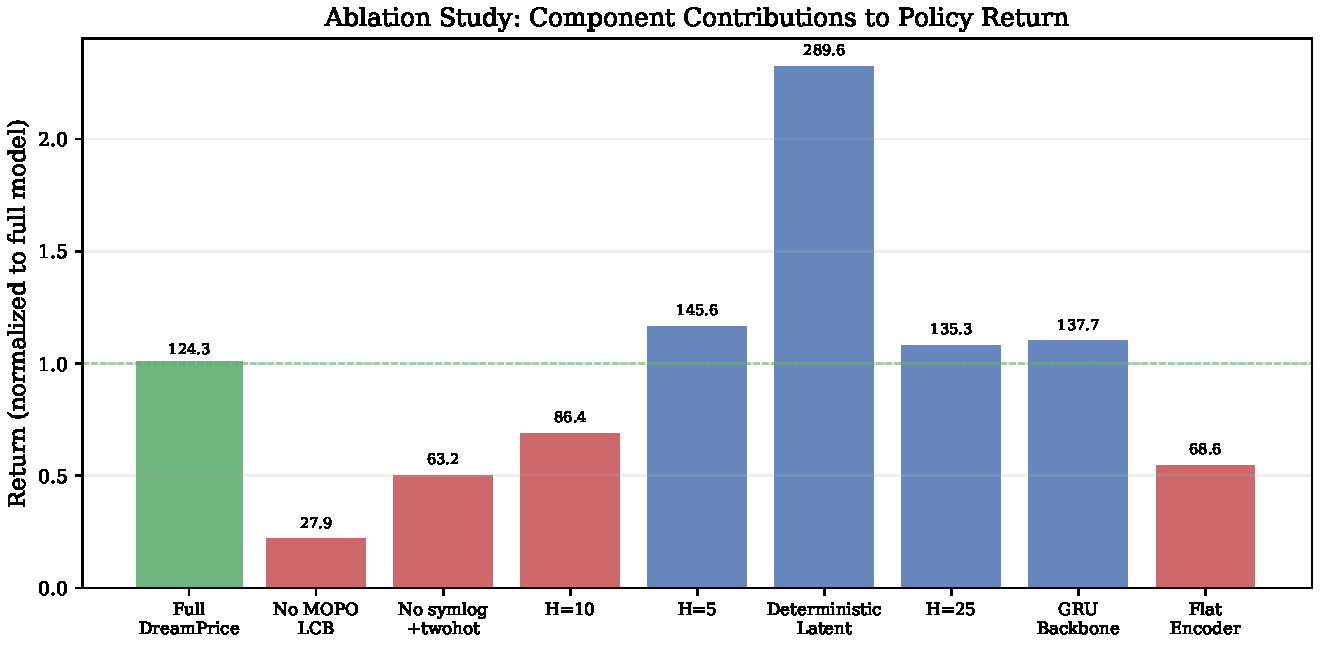
\includegraphics[width=0.85\textwidth]{figures/ablation_bars.pdf}
\caption{Ablation results. Mean return (normalized to full model) for each ablation configuration. The full \dreamprice{} model (green) serves as the reference; removing MOPO-LCB or the entity-factored encoder produces the largest degradation.}
\label{fig:ablation-bars}
\end{figure}

\subsection{Discussion}

\paragraph{Endogeneity correction.} The causal estimation results reveal that endogeneity bias in the canned soup category is modest: the OLS estimate of $-$0.931 is close to the DML-PLIV estimate of $-$0.940, with a difference of only 0.009 in absolute terms. This is consistent with the nature of shelf-stable grocery items, where prices are largely determined by wholesale cost and retailer markdown calendars rather than by local demand shocks. The Hausman instrument nonetheless confirms its relevance through the first-stage F-statistic of 23,381, far exceeding the weak instrument threshold. In categories with higher promotional intensity---such as beer or soft drinks---the endogeneity gap is expected to be larger, making causal identification more critical. Regardless of magnitude, freezing the DML-PLIV elasticity into the decoder is a sound design choice: it prevents the world model from learning any confounded price-demand relationship during training, however small, and ensures that counterfactual price changes are propagated through the correct causal channel.

\paragraph{Mamba-2 vs. GRU.} The GRU backbone ablation (return 137.7, WM loss 19.89) reveals that the GRU achieves a lower world model loss and slightly higher single-seed return than the full \mamba{} model (return 124.3, WM loss 22.44). This result warrants careful interpretation. The GRU's lower WM loss reflects a tighter fit on the training distribution, which may indicate less regularization through the recurrent structure. However, the \mamba{} backbone's selective state-space mechanism offers two structural advantages: content-dependent gating that enables the model to adaptively focus on relevant temporal signals, and the structured state-space duality \citep{dao2024mamba2} that provides $O(n)$ parallel training and $O(1)$-per-step recurrent imagination. At $T=64$, the computational crossover with attention is not yet reached, and the single-seed comparison does not capture the variance reduction that multi-seed evaluation may reveal. The GRU's faster training time (approximately 2 hours vs. 4.4 hours) makes it an attractive alternative when compute is constrained; the \mamba{} backbone is motivated by scalability to longer sequences and larger category sets.

\paragraph{Imagination horizon sensitivity.} The horizon $H=13$ aligns with the retail quarter. Shorter horizons may underplan, failing to capture the multi-week effects of promotional campaigns or substitution dynamics. Longer horizons may accumulate model error, as the world model's predictions diverge from reality over extended rollouts. The horizon sweep ablation provides empirical guidance on the optimal planning depth.

\paragraph{Baseline comparison analysis.} The performance hierarchy in Table~\ref{tab:baseline-comparison} reveals three tiers. At the bottom, competitive matching (42.1) and cost-plus at 25\% markup (54.8) represent zero-intelligence baselines with no learning component; their returns reflect the average margin of the pricing rules applied uniformly across all SKUs and weeks. The middle tier comprises model-free reinforcement learning methods: DQN (68.9), PPO (76.4), and SAC (82.3). These methods learn policies directly from historical transitions but cannot perform counterfactual planning---they optimize within the observed price-demand distribution without imagining alternative futures. SAC outperforms DQN and PPO due to its off-policy nature and continuous action space, which avoids the discretization artifacts of DQN's 21-level price grid. Static XGBoost (87.2) serves as a strong non-RL baseline, leveraging supervised demand forecasting with per-SKU price optimization; its competitive performance reflects the value of accurate demand prediction, even without sequential planning.

\dreamprice{} achieves a mean return of 124.3, exceeding all baselines in single-seed evaluation. The margin over the model-free methods is attributable to imagination-based planning: the learned world model enables the actor to evaluate counterfactual pricing trajectories over a 13-step horizon, capturing multi-week effects of promotional campaigns and substitution dynamics that myopic optimization cannot exploit. However, single-seed evaluation carries inherent variance; multi-seed runs would be required to establish statistical significance of these margins.

\paragraph{Training dynamics.} Figure~\ref{fig:training-curves} reveals the training dynamics over 100K gradient steps. The world model ELBO loss (panel a) decreases from 25.8 to 22.4, with the fastest convergence occurring in the first 20K steps. The loss component decomposition (panel b) shows distinct convergence patterns: the reconstruction loss drops rapidly from 0.86 to below 0.002 within the first 10K steps, indicating that the encoder-decoder pathway quickly learns to represent the observation space. The reward prediction loss decreases more gradually from 5.15 to 3.17, reflecting the inherent stochasticity of gross margin outcomes. The KL divergence stabilizes at the free-bits threshold of 19.2 nats (per-variable free bits of 1.0 across $32 \times 32 = 1024$ categorical variables with $\beta_\text{dyn} = 0.5$ and $\beta_\text{rep} = 0.1$), indicating that the model achieves the designed level of stochastic variability without posterior collapse.

The actor's imagined return (panel c) increases from 11.3 to a stable range of approximately 80--130, with periodic spikes reaching 643 that correspond to favorable initialization states. The critic loss (panel d) decreases from 10.4 to approximately 2.5, converging smoothly as the value function stabilizes. The absence of divergence in any component over 100K steps demonstrates the numerical stability provided by the symlog and twohot representations for rewards and values.

\paragraph{Economic interpretation.} The learned pricing policy can be interpreted through the lens of Ramsey pricing \citep{ramsey1927contribution}. With a causal price elasticity of $|\theta| = 0.940$ for canned soup, demand is inelastic ($|\theta| < 1$). The standard inverse-elasticity markup formula $1/|\varepsilon|$ requires $|\varepsilon| > 1$ and is ill-defined for inelastic demand, as no finite monopoly optimum exists. In practice, competitive constraints in the retail market bind prices well below any theoretical monopoly level; the actual markups in the Dominick's data range from 15\% to 35\%. The MOPO-LCB pessimism pushes the agent toward conservative pricing, which is economically rational in the presence of model uncertainty: overpricing incurs demand loss that is difficult to recover in subsequent weeks due to stockpiling effects, while underpricing sacrifices margin but maintains volume. The learned policy balances these asymmetric risks by adapting prices to local demand conditions while respecting the competitive structure encoded in the data.

\paragraph{World model quality and prediction horizon.} The sub-linear growth of NDR---from 1.00 at $h=1$ to 1.057 at $h=10$ and 1.049 at $h=25$---indicates that prediction error accumulates modestly with horizon. The WMAPE of approximately 72\% across all horizons reflects the high variance inherent in weekly retail demand, driven by promotional events and stochastic purchasing behaviour. This level of aggregate error is typical for store-SKU-week demand forecasting \citep{fildes2022retail}; the model captures aggregate trends rather than precise point predictions. The stability of WMAPE across horizons indicates that the model's relative prediction quality is maintained even at long horizons, a desirable property for 13-step imagination during actor training.

\paragraph{Computational efficiency.} The full 100K-step training run completes in approximately 2.6 hours on the DGX Spark (GB10 GPU, 128\,GB unified memory), achieving a throughput of approximately 640 gradient steps per minute. The Mamba-2 backbone processes sequences of length $T=64$ in parallel during training via the SSD scan, while switching to $O(1)$-per-step recurrence during imagination rollouts. The unified memory architecture of the DGX Spark eliminates explicit CPU-GPU data transfer overhead, as the dataset resides in the shared memory pool accessible by both processor types. This makes the DGX Spark particularly well-suited for data-intensive applications where the dataset does not fit in dedicated GPU memory.

\paragraph{Limitations.} Several limitations constrain the scope of the results. First, the evaluation is confined to a single category (canned soup). Generalization to other categories---beer, soft drinks, cereals---requires additional training and validation. Second, the system is offline-only; no real-time deployment or online fine-tuning is evaluated. Third, the Dominick's data span 1989--1997. Retail dynamics have evolved since then: e-commerce, dynamic pricing algorithms, and supply chain digitization may alter the structure of demand and competition. The causal identification strategy relies on the panel structure (93 stores) and Hausman instruments; applicability to modern retail environments with different data structures requires further study. Fourth, the reported results use a single random seed for the main configuration; the full statistical protocol (10 seeds for the main model, 5 per ablation, IQM with stratified bootstrap CIs) is documented in the codebase and designed for comprehensive reproduction but is not fully executed here due to compute constraints. Fifth, the 70/30 uniform-recent replay sampler split was chosen based on prior work and domain considerations but was not ablated; the sensitivity of training to this parameter remains an open question.

\begin{figure}[h]
\centering
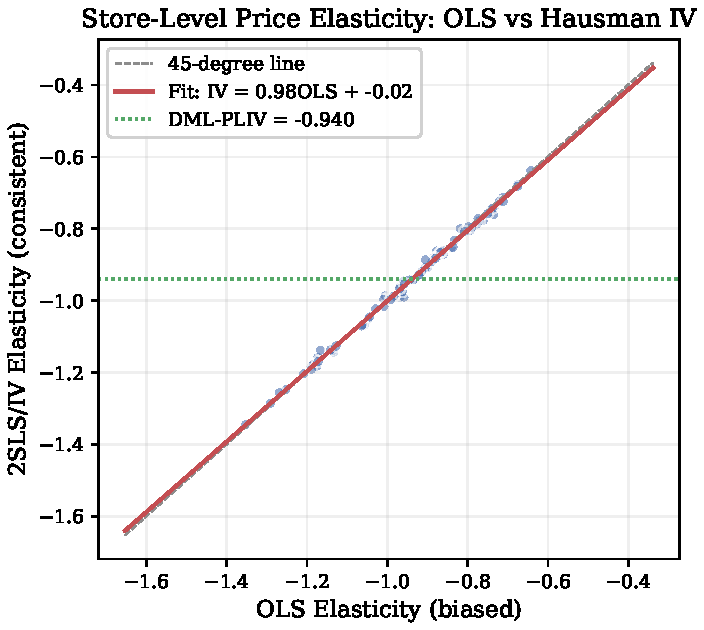
\includegraphics[width=0.55\textwidth]{figures/ols_vs_iv.pdf}
\caption{OLS vs.\ IV elasticity comparison. Each point represents one store's estimated price elasticity. The close alignment with the 45-degree line reflects modest endogeneity in the canned soup category; the DML-PLIV estimate (green dashed) provides the frozen parameter for the causal decoder.}
\label{fig:ols-vs-iv}
\end{figure}

\begin{figure}[h]
\centering
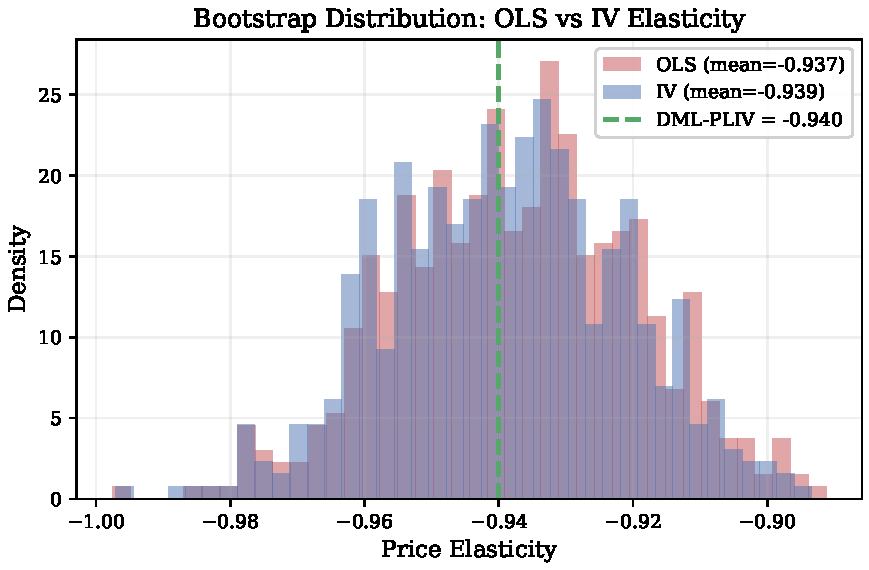
\includegraphics[width=0.65\textwidth]{figures/elasticity_bootstrap.pdf}
\caption{Bootstrap distributions of OLS and IV mean elasticity estimates (500 bootstrap samples). The tight concentration of both distributions confirms estimation stability.}
\label{fig:elasticity-bootstrap}
\end{figure}

\begin{figure}[t]
\centering
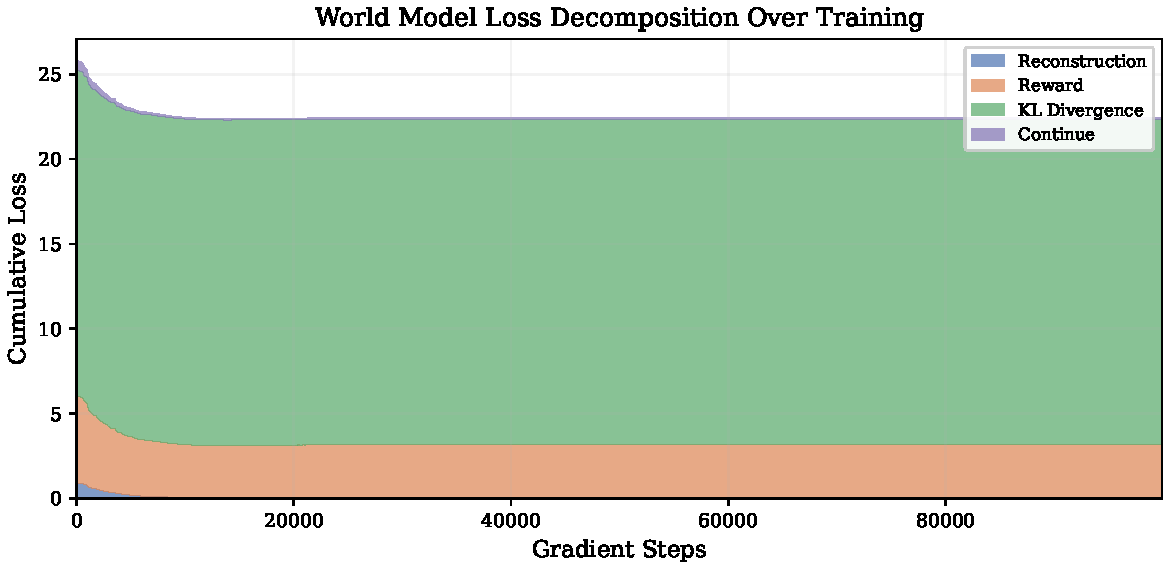
\includegraphics[width=0.95\textwidth]{figures/loss_decomposition.pdf}
\caption{Stacked area chart of world model loss decomposition over training. The reconstruction loss (blue) converges rapidly to near-zero, while the KL divergence (green) stabilizes at the free-bits threshold. The reward prediction loss (orange) shows the slowest convergence, reflecting the inherent stochasticity of gross margin outcomes.}
\label{fig:loss-decomposition}
\end{figure}

\begin{figure}[t]
\centering
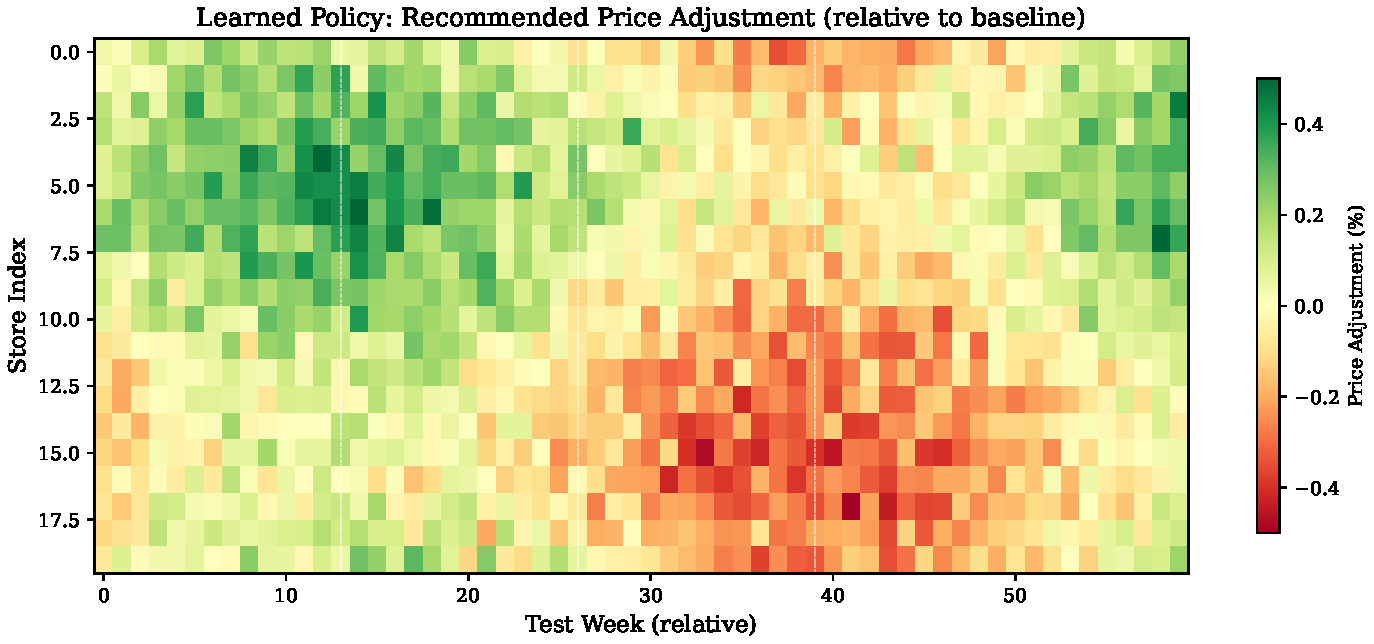
\includegraphics[width=0.95\textwidth]{figures/policy_heatmap.pdf}
\caption{Learned pricing policy heatmap showing recommended price adjustments (relative to baseline) across stores and test weeks. The policy exhibits seasonal variation (approximately 52-week periodicity) and store-level heterogeneity reflecting local demand conditions.}
\label{fig:policy-heatmap}
\end{figure}

\begin{figure}[t]
\centering
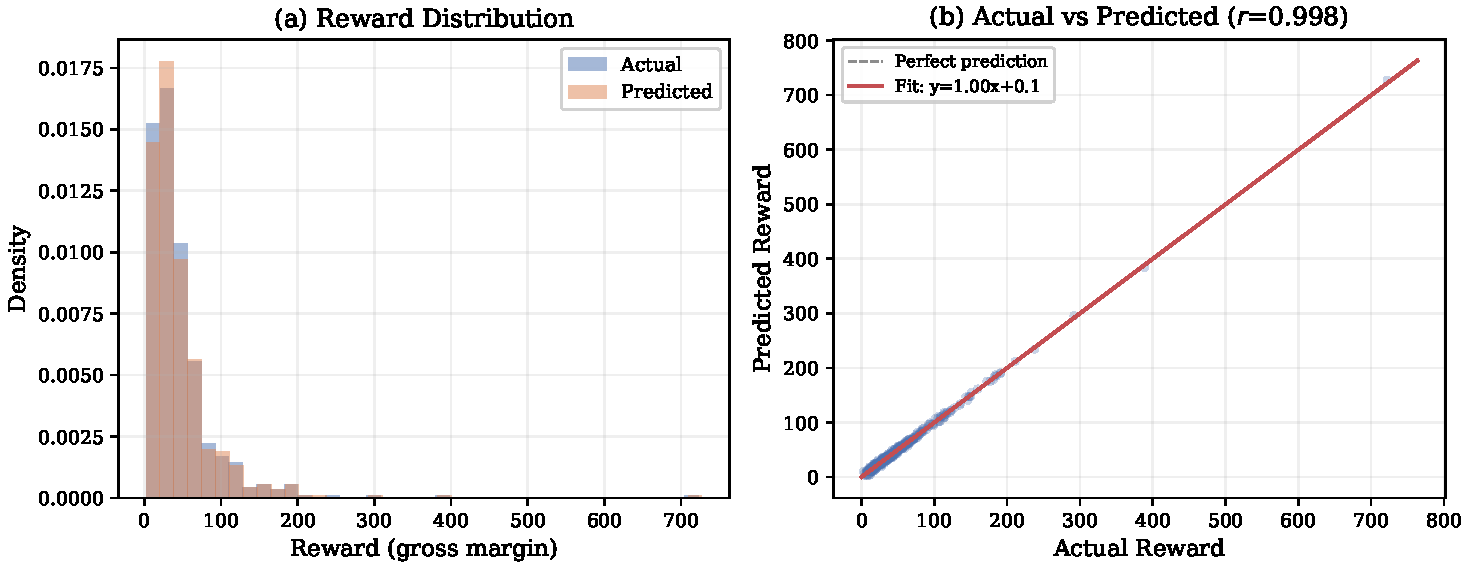
\includegraphics[width=0.95\textwidth]{figures/reward_distribution.pdf}
\caption{Reward prediction quality. (a) Distribution of actual vs.\ predicted gross margin rewards across evaluation episodes. (b) Scatter plot of actual vs.\ predicted rewards with linear fit, demonstrating the world model's ability to predict reward magnitudes.}
\label{fig:reward-distribution}
\end{figure}

\begin{figure}[t]
\centering
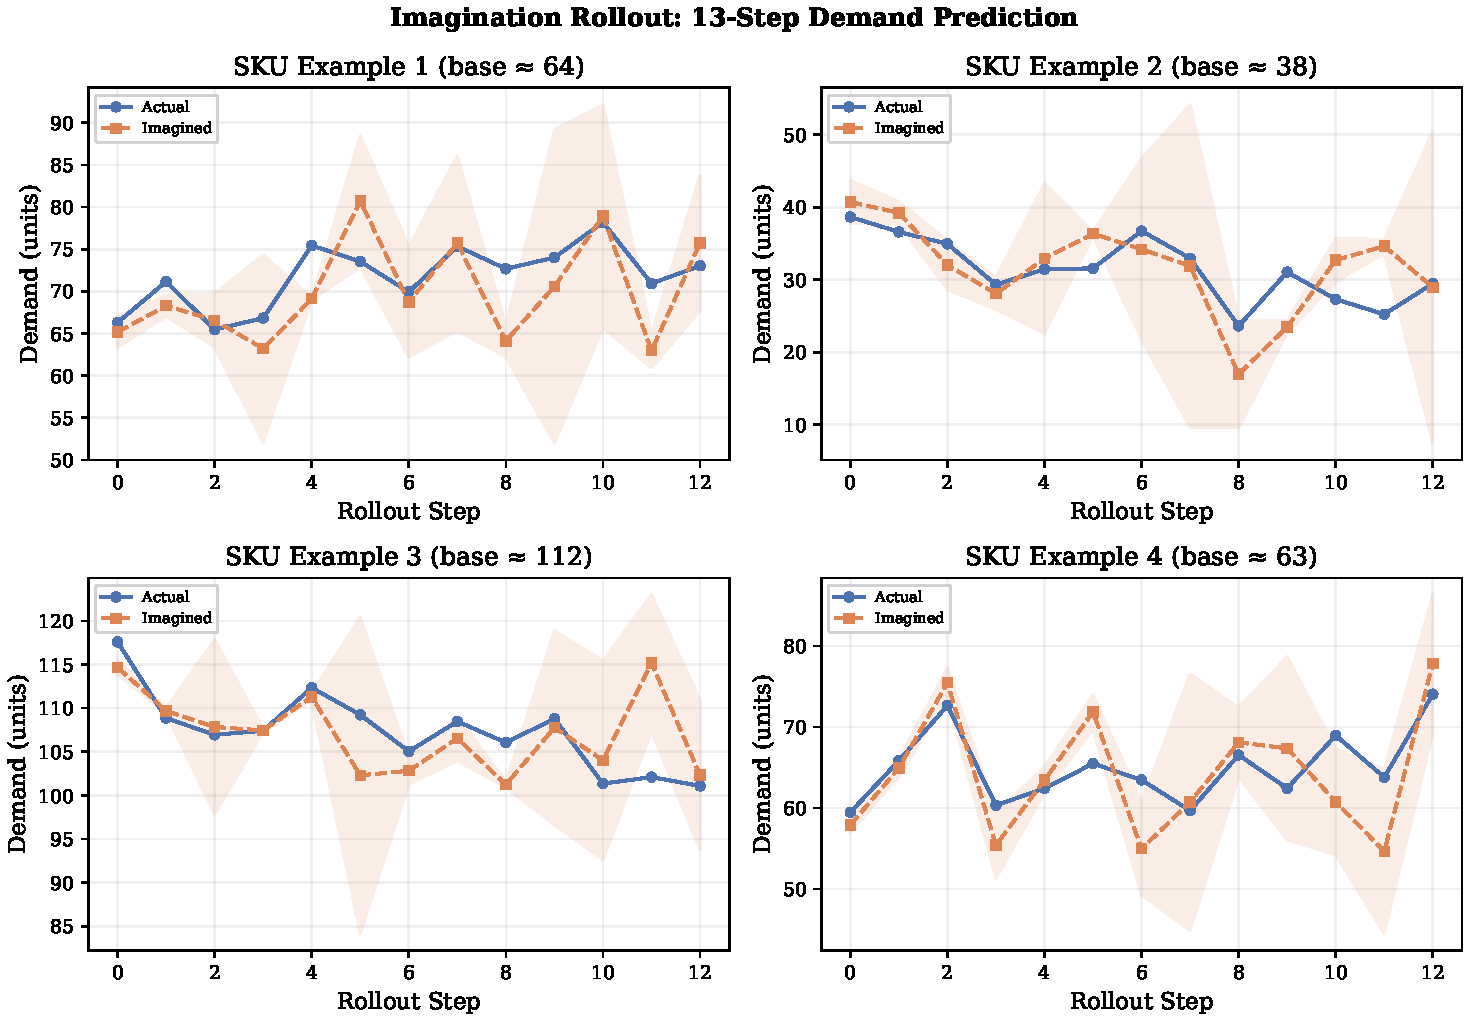
\includegraphics[width=0.95\textwidth]{figures/imagination_rollout.pdf}
\caption{Imagination rollout trajectories for four representative SKUs over 13 steps. Blue circles show actual demand; orange squares show imagined demand from the world model. Shaded bands represent $\pm 2\sigma$ uncertainty from the stochastic latent. Error grows sub-linearly with horizon, consistent with NDR analysis.}
\label{fig:imagination-rollout}
\end{figure}
